%Notes by Harsh Mistry 
%CS 444
%based on Template from : https://www.cs.cmu.edu/~ggordon/10725-F12/template.tex

\documentclass{article}
\setlength{\oddsidemargin}{0.25 in}
\setlength{\evensidemargin}{-0.25 in}
\setlength{\topmargin}{-0.6 in}
\setlength{\textwidth}{6.5 in}
\setlength{\textheight}{8.5 in}
\setlength{\headsep}{0.75 in}
\setlength{\parindent}{0 in}
\setlength{\parskip}{0.1 in}
\usepackage{amsfonts,graphicx, amssymb}
\usepackage[fleqn]{amsmath}
\usepackage{fixltx2e}
\usepackage{color}
\usepackage{tcolorbox}
\usepackage{lipsum}
\usepackage{listings}
\graphicspath{ {./images/} }
\usepackage{scrextend}
\tcbuselibrary{skins,breakable}
\usetikzlibrary{shadings,shadows}
\newcounter{lecnum}
\renewcommand{\thepage}{\thelecnum-\arabic{page}}
\renewcommand{\thesection}{\thelecnum.\arabic{section}}
\renewcommand{\theequation}{\thelecnum.\arabic{equation}}
\renewcommand{\thefigure}{\thelecnum.\arabic{figure}}
\renewcommand{\thetable}{\thelecnum.\arabic{table}}
\newcommand{\lecture}[4]{
   \pagestyle{myheadings}
   \thispagestyle{plain}
   \newpage
   \setcounter{lecnum}{#1}
   \setcounter{page}{1}
   
   
%Info Box 
   \begin{center}
   \framebox{
      \vbox{\vspace{2mm}
    \hbox to 6.28in { {\bf CS 444 - Compiler Construction 
	\hfill Winter 2020} }
       \vspace{4mm}
       \hbox to 6.28in { {\Large \hfill Lecture #1: #2  \hfill} }
       \vspace{2mm}
       \hbox to 6.28in { {\it Lecturer: #3 \hfill Notes By: #4} }
      \vspace{2mm}}
   }
   \end{center}
   
   \markboth{Lecture #1: #2}{Lecture #1: #2}



 
}

\renewcommand{\cite}[1]{[#1]}
\def\beginrefs{\begin{list}%
        {[\arabic{equation}]}{\usecounter{equation}
         \setlength{\leftmargin}{2.0truecm}\setlength{\labelsep}{0.4truecm}%
         \setlength{\labelwidth}{1.6truecm}}}
\def\endrefs{\end{list}}
\def\bibentry#1{\item[\hbox{[#1]}]}

\newcommand{\fig}[3]{
			\vspace{#2}
			\begin{center}
			Figure \thelecnum.#1:~#3
			\end{center}
	}
	
\newcommand{\pipe}{\(\mid\)}
\newcommand{\ctr}{\(\wedge\)}

\newtheorem{theorem}{Theorem}[lecnum]
\newtheorem{lemma}[theorem]{Lemma}
\newtheorem{ex}[theorem]{Example}
\newtheorem{proposition}[theorem]{Proposition}
\newtheorem{claim}[theorem]{Claim}
\newtheorem{corollary}[theorem]{Corollary}
\newtheorem{definition}[theorem]{Definition}
\newenvironment{proof}{{\bf Proof:}}{\hfill\rule{2mm}{2mm}}
\newcommand\E{\mathbb{E}}

%color definitions :
\definecolor{darkred}{rgb}{0.55, 0.0, 0.0}
\definecolor{lightcoral}{rgb}{0.94, 0.5, 0.5}
\definecolor{tomato}{rgb}{1.0, 0.39, 0.28}
\definecolor{lightgray}{rgb}{.9,.9,.9}
\definecolor{darkgray}{rgb}{.4,.4,.4}
\definecolor{purple}{rgb}{0.65, 0.12, 0.82}
\definecolor{lightgreen}{rgb}{0.56, 0.93, 0.56}
\definecolor{darkgreen}{rgb}{0.0, 0.2, 0.13}
\definecolor{limegreen}{rgb}{0.2, 0.8, 0.2}
\definecolor{lightblue}{rgb}{0.68, 0.85, 0.9}
\definecolor{darkblue}{rgb}{0.0, 0.0, 0.55}


%Environments
\newenvironment{exblock}[1]{%
    \tcolorbox[beamer,%
    noparskip,breakable,
    colback=lightgreen,colframe=darkgreen,%
    colbacklower=limegreen!75!lightgreen,%
    title=#1]}%
    {\endtcolorbox}

\newenvironment{ablock}[1]{%
    \tcolorbox[beamer,%
    noparskip,breakable,
    colback=lightcoral,colframe=darkred,%
    colbacklower=tomato!75!lightcoral,%
    title=#1]}%
    {\endtcolorbox}

\newenvironment{cblock}[1]{%
    \tcolorbox[beamer,%
    noparskip,breakable,
    colback=lightblue,colframe=darkblue,%
    colbacklower=darkblue!75!lightblue,%
    title=#1]}%
    {\endtcolorbox}


%Languages
\lstdefinelanguage{JavaScript}{
  keywords={typeof, new, true, false, catch, function, return, null, catch, switch, var, if, in,  fi, while, do, else, case, break},
  keywordstyle=\color{blue}\bfseries,
  ndkeywords={class, export, boolean, throw, implements, import, this},
  ndkeywordstyle=\color{darkgray}\bfseries,
  identifierstyle=\color{black},
  sensitive=false,
  comment=[l]{//},
  morecomment=[s]{/*}{*/},
  commentstyle=\color{purple}\ttfamily,
  stringstyle=\color{red}\ttfamily,
  morestring=[b]',
  morestring=[b]"
}

%Listings
\lstset{
   language=JavaScript,
   backgroundcolor=\color{lightgray},
   extendedchars=true,
   basicstyle=\footnotesize\ttfamily,
   showstringspaces=false,
   showspaces=false,
   numbers=left,
   numberstyle=\footnotesize,
   numbersep=9pt,
   tabsize=2,
   breaklines=true,
   showtabs=false,
   captionpos=b
}


%Start of Document 
\begin{document}

\lecture{9}{February 3rd , 2020}{Ond\u{r}ej Lhot\'{a}k}{Harsh Mistry}

\section{Analysis Continued}

\subsection{Parsing Continued}

\subsubsection{LR(1) NFA}
 \textbf{Note:} (H : I), I is the look ahead symbol in this context
 \begin{itemize}
 \item \(\Sigma = T \cup N \)
 \item \( Q = \{ A \rightarrow \alpha \cdot \beta : a | A \rightarrow \alpha \beta \in R \}\)
 \item \(q_0 = S^\prime \rightarrow s \$ : \$\) 
 \item \(A = Q\)
 \item \(\delta ( A \rightarrow \alpha \cdot B \beta : a, \epsilon ) = \{ B \rightarrow \cdot \gamma : b | B \rightarrow \gamma \in R \text{ and } b \in first(\beta a) \}\)
 \item \(\delta ( A \rightarrow \alpha \cdot X \beta : a, X) = \{ A \rightarrow \alpha X \cdot \beta : a  \} \)
 \item If NFA ends up in \(B \rightarrow \gamma \cdot : b \) on stack \(\beta \gamma\), then \(B \rightarrow \gamma \in Reduce(\beta \gamma, b)\) because the NFA would also accept \(\beta \beta b\)
 \end{itemize}
 
 \subsubsection{LR(1) DFA}
 
 \begin{itemize}
 \item S-R: if DFA state contains \(A \rightarrow \gamma \cdot : a \) and \(B \rightarrow \alpha \cdot a \beta : b \)
 \item R-R: if DFA state contains \(A \rightarrow \gamma \cdot : a\) and \(B \rightarrow \delta \cdot : a \)
 \end{itemize}
 \begin{ex}-\\
 \textbf{Grammar:}
 \begin{itemize}
 \item \(S^ \prime \rightarrow \cdot S \$\)
 \item \(S \rightarrow \cdot a : \$\)
 \item \(S \rightarrow \cdot E = E : \$\)
 \item \(E \rightarrow \cdot a : = \)
 \item \(E \rightarrow \cdot \star E : = \)
 \end{itemize}
 \begin{center}
 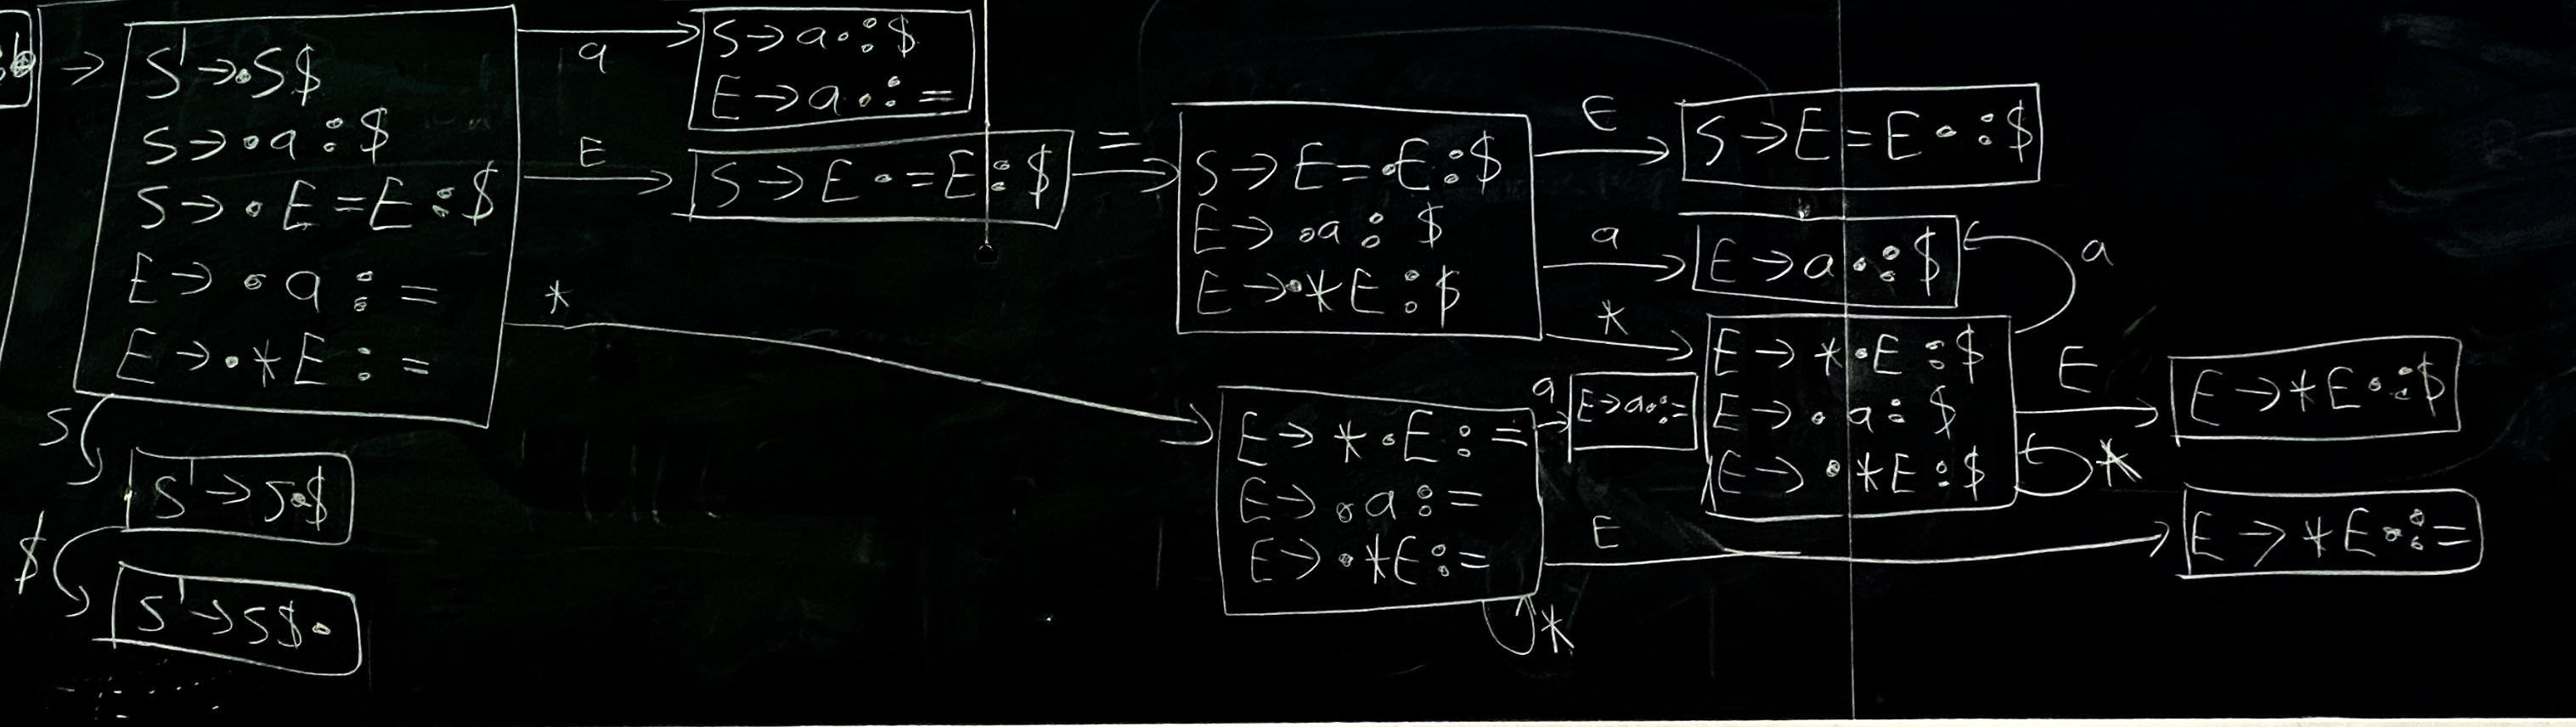
\includegraphics[scale=0.15]{10}
 \end{center}
 \end{ex}
 
 \begin{itemize}
 \item The example highlights that LR(1) DFA's are often big and occupy more than 1Mb. 
 \item LALR(1): uses LR(0) DFA with local follow sets in states. 
 \end{itemize}

\subsubsection{LALR(1)}
\begin{definition} 
\(cove(q) = \{ A \rightarrow \cdot \beta | A \rightarrow a \cdot \beta : a \in q\}\) 
\end{definition}

\begin{exblock}{Fact}
If we replace each LR(1) DFA state with its cove, we get LR(0) DFA
\end{exblock}

\begin{cblock}{Idea}
For each item (NFA  state) in the LR(0) DFA state, use corresponding look-a-ahead symbols from LR(1) DFA states
\end{cblock}


\end{document}







